% Documentation/Structure:
%     + Table of Contents
%     + Preface
%         - Legal Notice
%     + Problem
%     + To-be Concept
%         - Functional Concept
%         - Technical Concept
%     + Time line
%     + Implementation
%         - Problems and Solutions
%         - Changes
%     + Quality Assurance
%         - Testing
%         - Known Issues
%     + List of Figures
%     + List of Tables


\documentclass[12pt]{scrreprt}

\usepackage[english]{babel}
\usepackage{color}
\usepackage{float}
\usepackage{fancyhdr}
\usepackage{fancyref}
\usepackage[T1]{fontenc}
\usepackage{graphicx}
\usepackage{hyperref}
\usepackage[utf8]{inputenc}
\usepackage{longtable}
\usepackage{nameref}
\usepackage{rotating}
% Removes some false-positive warnings.
\usepackage{scrhack}
\usepackage{tabularx}

\title{Game Database}
\subtitle{Documentation}
\author{LCManager Group\\Dominik Cech\\Fabian Damken\\Stefan Müller\\Tobias Bahrmann}
\date{\today}
\makeatletter
\def\@brand{../../gdb-web-control/src/main/resources/static/images/brand/brand_512.png}
\makeatother

\makeatletter
\renewcommand\maketitle{%
	\begin{center}
		\thispagestyle{empty}
		\textsc{\LARGE}\\[2cm]
		\textsc{\Huge \@title}\\[1cm]
		\textsf{\normalsize \@subtitle}\\[1cm]
		\textsf{\small by}\\[1.5cm]
		\textsc{\large \@author}\\[0.25cm]
		\textsc{\large \today}\\[1.75cm]
		\includegraphics[width=0.5\textwidth]{\@brand}
	\end{center}
}
\makeatother

\makeatletter
\def\@pagestyle{
	\fancyhf{}
	\lhead{\includegraphics[height=0.05\textheight]{\@brand}}
	\chead{\leftmark}
	\rhead{\@date}
	\rfoot{Page \thepage}
}
\fancypagestyle{plain}{\@pagestyle}
\@pagestyle
\pagestyle{fancy}
\makeatother

\definecolor{gray}{rgb}{0.6, 0.6, 0.6}
\definecolor{light-red}{rgb}{1, 0.3, 0}
\definecolor{light-blue}{rgb}{0, 0.5, 1}
\definecolor{dark-red}{rgb}{0.6, 0, 0}
\definecolor{dark-green}{rgb}{0, 0.6, 0}
\definecolor{orange}{rgb}{1, 0.8, 0}

\setcounter{secnumdepth}{5}
\setcounter{tocdepth}{1}

\begin{document}
	\maketitle
	\tableofcontents

	\chapter{Preface}
		\label{ch:preface}

		\section{Legal Notice}
			\label{sec:preface_legal_notice}

			\begin{verbatim}
Game Database

Copyright (C) 2016 - 2016 LCManager Group

Licensed under the Apache License, Version 2.0 (the
"License");
you may not use this file except in compliance with the
License. You may obtain a copy of the License at

     http://www.apache.org/licenses/LICENSE-2.0

Unless required by applicable law or agreed to in writing,
software distributed under the License is distributed on an
"AS IS" BASIS, WITHOUT WARRANTIES OR CONDITIONS OF ANY
KIND, either express or implied.
See the License for the specific language governing
permissions and limitations under the License.
			\end{verbatim}

			\rule{\linewidth}{1pt}

			\begin{verbatim}
This document, the project configuration including the IDE
configuration, all tool configuration and application
configuration, the source code including the production
code an the test code written in Java and Groovy, all
production resources and test resources, all binary
derivatives and executable files, the documentation and the
specification and all other files, folder, links and other
file system entries are subject of the license.
			\end{verbatim}

	\chapter{Problem}
		\label{ch:problem}

		Most of the time the system requirements of games are very confusing and hard to understand. This causes some user not to buy any game because they do not understand the system requirements and frustrates them because they want to play the game. Some user may act risky and buy the game, no matter whether they know that their system can run the game or not. This causes them to be unhappy if the game does not run and they will blame either the game, the publisher or the developer because they did not point out the requirements correctly (if the user thinks he understood the requirements correctly).

		The complexity of the system requirements merge together with the complexity of technology in general. That is the technical specifications on the one hand and the product names on the other hand.
		\\
		For example: Which graphics card is better (for gaming, if course): The NVIDIA GT 7600 or the NVIDIA GTX 970? The NVIDIA GTX 970 is better. This is a good example that it is impossible to compare products just by their name or the numbers in their name. You must compare the technical specifications to see which one is better and this procedure is really complex.



	\chapter{To-be Concept}
		\label{ch:tb-concept}

		This chapter describes how the Game Database solves all problems shown above and how that is implemented.

		\section{Functional Concept}
			\label{sec:tb-concept_functional}

			During the creation of the Game Database the focus was to solve all shown problems in a very simple and user-friendly way.

			Therefore the Game Database consists of a nice-looking user interface which can be reached through the browser which provides a simple interface for searching for games. Once a game was found and the user decides he wants to read the game details the system requirements are compared to the primary system that the user has saved. The result of this comparison is displayed as a speedometer where '0' means that the game cannot be ran and '100' means that the system completely fulfills the requirements. Minimum and recommended requirements are separated from each other as some games do not provide recommended requirements.

			As said above, a user can save one or more systems and can mark one as the primary system. The primary system is the only system that gets compared to any game instantly when the game details are loaded. For any other system, the user has to manually select it. 

			This brings us to to the user management. A user has to register by providing a unique user name, a display name and a password in order to be able to save any system. If not, a comparison is not possible as no system is available.

			The Game Database contains data for more than 8000 games and supports more than 1000 graphics cards and processors produced by AMD, Intel and NVIDIA.


		\section{Technical Concept}
			\label{sec:tb-concept_technical}

			\subsection{Basic Concept}
				\label{subsec:tb-concept_technical_basic}

				The basic concept behind the Game Database is to connect to third-party services like Steam and NVIDIA in order to retrieve the required data for the comparison. That means that only some games are saved directly in the Game Database and most of the data is loaded from Steam.
				\\
				Also, the data about graphics cards and processors (e.g. the clock speed) is loaded from the individual services for each brand.

			\subsection{Architectural Design}
				\label{subsec:tb-concept_technical_architectural-design}

				To structure these services the Game Database is split into the following modulesec:
				\begin{itemize}
					\item Game Database Base - Provides some basic utilities used in nearly every class of the Game Database.
					\item Game Database Service - Defines the basic services but does not implement them.
					\item Game Database Web Control - Controls the whole web interaction and defines the controllers that are handling the web requests.
					\item Game Database AMD Mapper - The mapper for the AMD service. This also implements some services of the Game Database Service.
					\item Game Database Intel Mapper - The mapper for the Intel service. This also implements some services of the Game Database Service.
					\item Game Database NVIDIA Mapper - The mapper for the NVIDIA service. This also implements some services of the Game Database Service.
					\item Game Database Steam Mapper - The mapper for the Steam service. This also implements some services of the Game Database Service.
					\item Game Database Service Implementation - Implements the Game Database Service by providing the connection to the database and by delegating most of the service calls to the branded implementations (e.g. the Game Database AMD Mapper).
					\item Game Database Application - Provides the actual implementation by wiring all modules together.
				\end{itemize}

				The figure \ref{fig:architecture_overview} (\nameref{fig:architecture_overview}) visualizes the modules described above and shows the communication between them.
				\begin{figure}[H]
					\label{fig:architecture_overview}
					\centering
					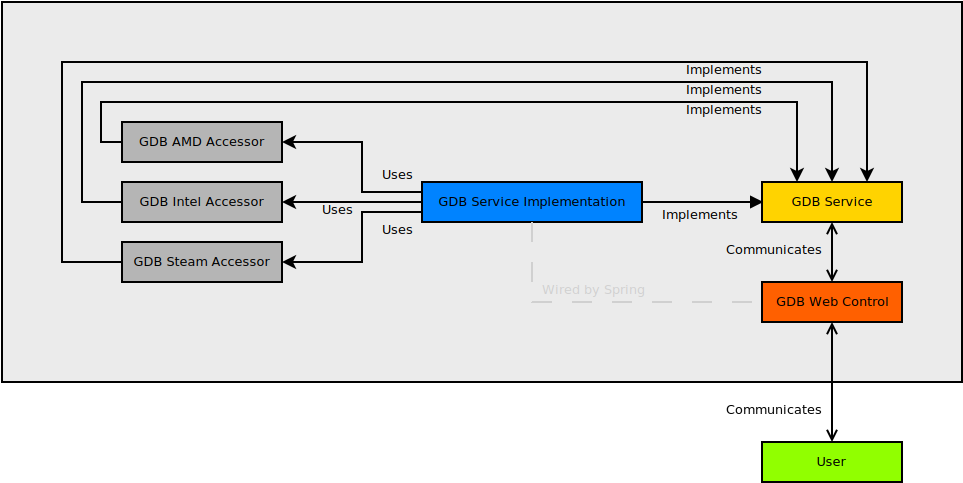
\includegraphics[width=\textwidth]{images/architecture/overview.png}
					\caption{Architecture - Overview}
				\end{figure}

				The \fcolorbox{black}{dark-green}{Green box} represents the user and is not a module of the Game Database.
				\\
				The \fcolorbox{black}{gray}{Big gray box} represents the Game Database Application as a container for all other modules.
				\\

				The splitting between the Game Database Service and its implementation (the Game Database Service Implementation) is necessary to prevent dependency cycles as the mappers depend on the Game Database Service and the Game Database Service would depend on them too, if the implementation where not split from the API specification (the Game Database Service).

			\subsection{Framework Usage}
				\label{subsec:tb-concept_technical_framework-usage}

				To run the application and to wire the modules together the Spring Framework is used. As the Spring Framework provides lots of single frameworks, only a few are used (this is a minified list, for a complete list please lookup \ref{sec:appendix_dependencies} (\nameref{sec:appendix_dependencies})):
				\begin{itemize}
					\item Spring AOP - Used for aspect-oriented programming.
					\item Spring Beans - Used for defining the beans and enable the dependency injection.
					\item Spring Boot - Used to boot the application.
					\item Spring Boot Actuator - Enables some utility pages.
					\item Spring Boot Autoconfigure - Configures the application automatically (mostly).
					\item Spring Context - Enables autowiring and the component-scan.
					\item Spring Expression - Brings the Spring Expression Language (SpEL).
					\item Spring HATEOAS - Enables the usage of hypermedia REST APIs.
					\item Spring Instrument - Instruments the classes and enabled load-time weaving.
					\item Spring JDBC - Connects Spring Data (and MyBatis) with JDBC.
					\item Spring Security - Secures the application.
					\item Spring Test - Brings some utility classes for testing the application.
					\item Spring Transaction - Enables transaction management to communicate with the database.
					\item Spring Web MVC - Brings the model-view-controller paradigm to the application and the views.
				\end{itemize}

				The application is built on top of Spring Web MVC and is therefore split into the model (the database model), the controllers (which are putting the data to the view) and the view (which is represented by some Freemarker templates).

				As said the application uses a database. To connect the application to the database very easy, MyBatis is used. It works seamless with Spring Transaction and Spring at all and configures (mostly) automatically. But MyBatis is only used in the background in the Game Database Service Implementation and is not populated through the whole application but rather the Game Database Service builds a facade around it by defining lots of services of which some are implemented using MyBatis mappers.
				\\
				MySQL is used as the database as it is very lightweight and runs mostly on every system (but it is only required on the server side, of course).

			\subsection{Database Design}
				\label{subsec:tb-concept_technical_database-design}

				The database is structured as you can see in figure \ref{fig:database_model} (\nameref{fig:database_model}).
				\begin{sidewaysfigure}
					\label{fig:database_model}
					\centering
					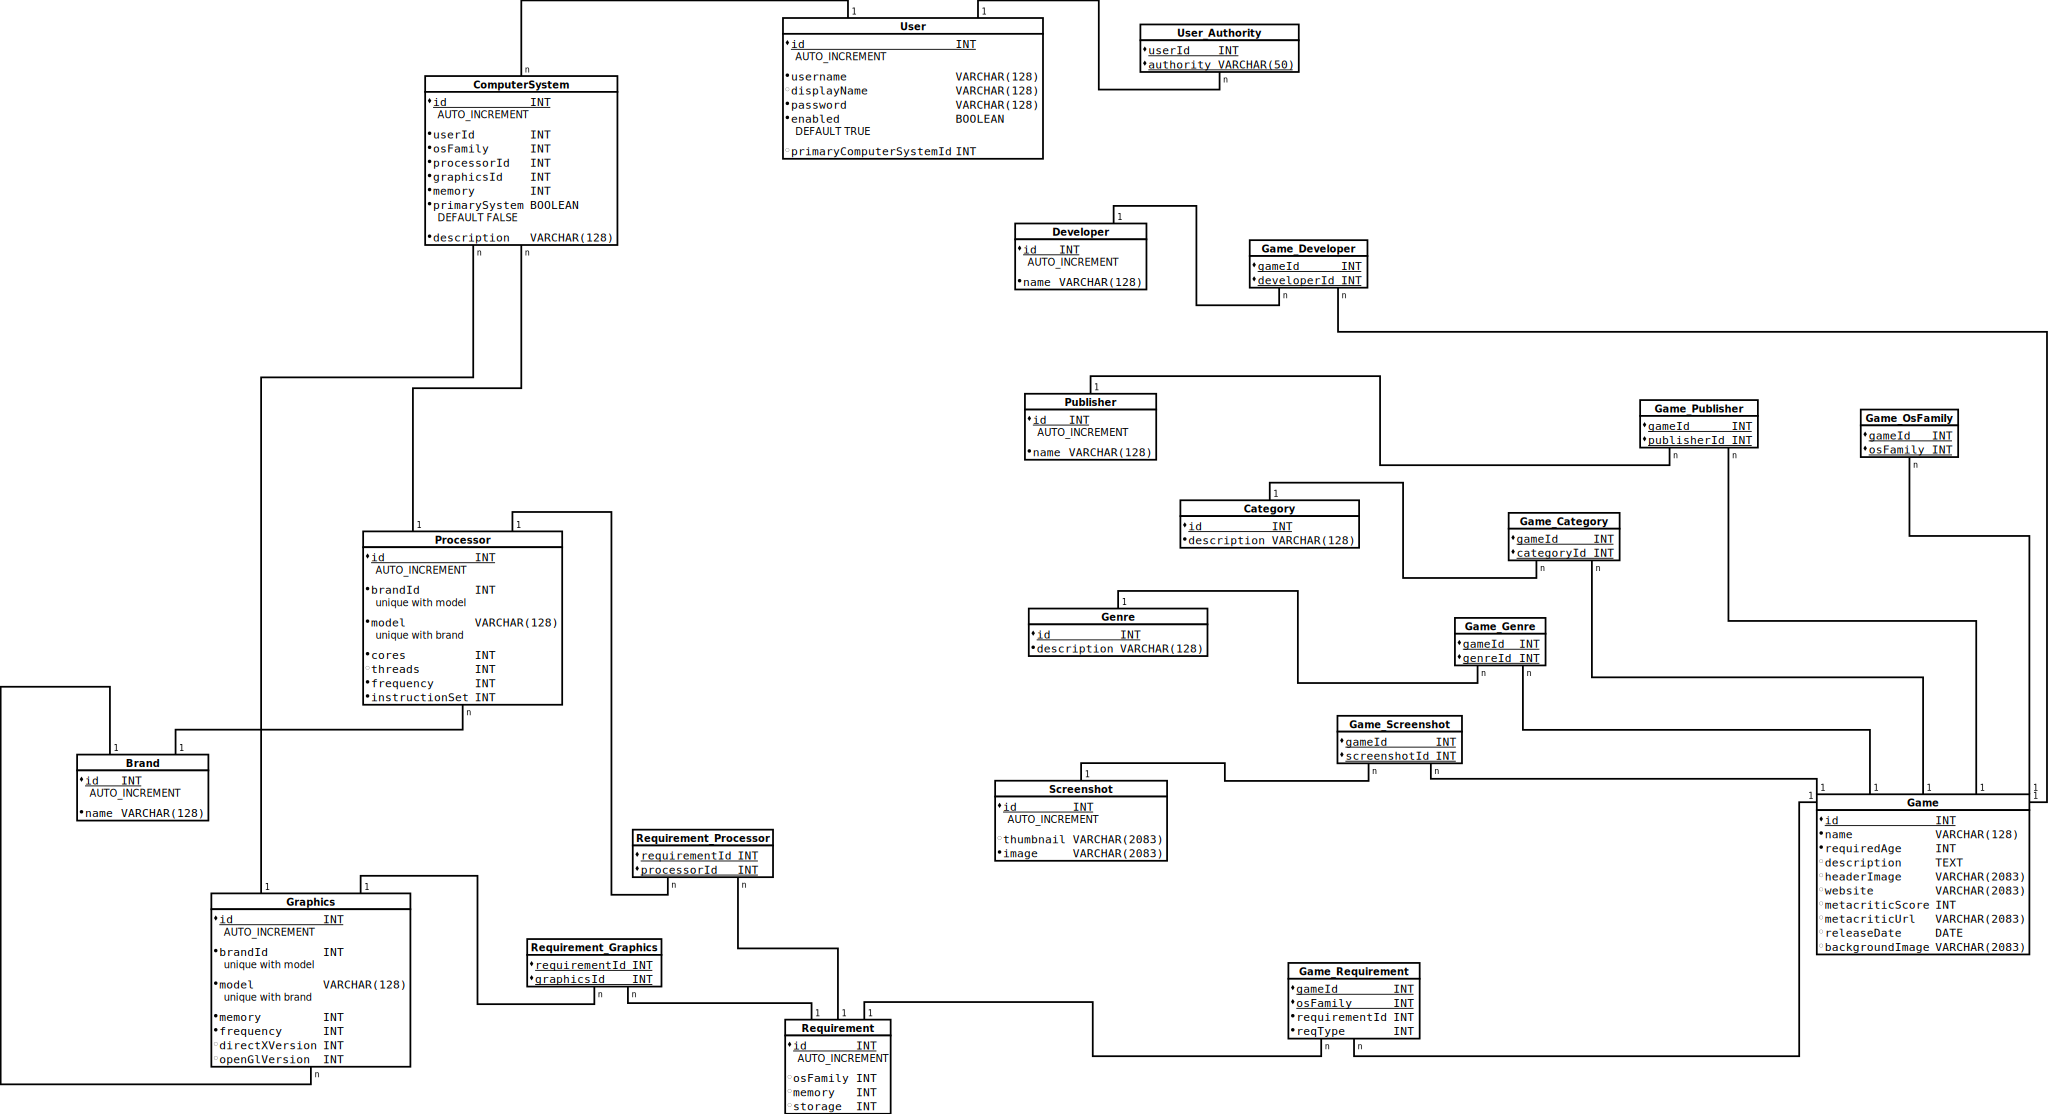
\includegraphics[width=\textwidth]{images/database/model.png}
					\caption{Database - Model}
				\end{sidewaysfigure}

			\subsection{Client Side}
				\label{subsec:tb-concept_technical_client-side}

				On the clients side the architecture is not as complicated as on the server side. It is basically built upon a model-view-controller principle where the model is the REST API provided by the server, the view is the actual HTML and the controller (-s) are defined by using AngularJS on the client side. The model-view-controller principle is used to strictly decouple the actual data from the view as this eases the development and allows the development of a single-page application.

				Also, Bootstrap is used in the client side to provide a basic styling for almost everything and to provide some reusable elements (e.g. a navigation). This eases the development a lot as it is not so cool to redesign the wheel.

				You can find a complete list of the dependencies on the client side in \ref{sec:appendix_dependencies-client} (\nameref{sec:appendix_dependencies-client}).



	\chapter{Time line}
		\label{ch:time-line}

		The project must be done within a bit more than one month (approximately 6-7 weeks). As this is a very short time, the time line is pretty strict and must be followed.

		The following things must be done before the actual development can be started:
		\begin{enumerate}
			\item Clarify the problem and the concept on how to solve the problem.
			\item Setting up the development environment. This includes:
				\begin{itemize}
					\item Setting up the Java Development Kit.
					\item Setting up Maven.
					\item Setting up Git.
					\item Setting up Eclipse.
					\item Configuring all above (e.g. configure the code formatter).
					\item Setting up MySQL.
				\end{itemize}
			\item Setting up the basic architecture and implement it. This includes:
				\begin{itemize}
					\item Creating the Git repository.
					\item Configuring Maven and the project modules.
					\item Including all dependencies.
				\end{itemize}
		\end{enumerate}

		After these basic steps the back-end has to be implemented. This includes the branded mappers, the database connection and anything else that is related to the back-end only. Parallel to that th development of the UI has to be started working on mock data produced by the back-end. The UID development includes the clarification of the design, the creation of a logo and the actual implementation.

		Also parallel to these steps the quality assurance is taking place watching for gross faults and minor details (e.g. some bad UI decisions).

		After everything of the above has been finished the final stabilization phase is started searching for issues and correcting them. This is a very important step that must not be skipped!

		Thereafter a final release can be published.



	\chapter{Implementation}
		\label{ch:implementation}

		The implementation takes place following the time line described in section \ref{ch:time-line}.

		\section{Problems and Solutions}
			\label{sec:implementation_problems}

			There where some problems during the development but must of them could be solved.
			\begin{table}[H]
				\label{tab:problems_solutions}
				\centering
				\begin{tabularx}{\textwidth}{ X | X }
					\multicolumn{1}{c |}{\textbf{Problem}} & \multicolumn{1}{c}{\textbf{Solution}}
					\\ \hline
					The release dates of games are formatter in a crazy way. Sometime they are simple 'May, 2016' but sometimes they are like 'q2 2016' which means quarter 2 of the year 2016. & The algorithm is now using a trial-and-error strategy to parse the date and replaces demented values like 'summer 2016' with actual months.
					\\ \\
					Searching for games is very slow as all details about all found games are loaded whenever the user searches for any game. The search takes about 15 seconds. & The search results have been trimmed down to only the necessary properties (e.g. the game name) which has fasten the search to approximately 1 second.
					\\ \\
					The NVIDIA mapper brought some surprises because not all graphics cards details can be retrieve using the same URL scheme. & the algorithm is now taking care of the type of the graphics card and checks whether it is a legacy graphics card as these are accesses in another way.
				\end{tabularx}
				\caption{Known Issues}
			\end{table}


		\section{Changes}
			\label{sec:implementation_changes}

			Since \today, no changes on the to-be concept took place.



	\chapter{Quality Assurance}
		\label{ch:qa}

		The quality assurance is applied as described in the time line described in section \ref{ch:time-line}.

		\section{Testing}
			\label{sec:qa_testing}

			The testing of the Game Database is completely automatized and no human has to touch it. However its usability was tested by people that are not related to the project team in any way to assure that it is usable.

			As tests both unit tests and integration tests are taking place both using modern technologies like Spock (for unit tests) and Selenium (for integration tests). Thanks to Spring Boot and Sprint Test, the integration testing is very simple.


		\section{Known Issues}
			\label{sec:qa_issues}

			This list contains known issues we are working on. When you recognize and issue, please send an E-Mail to \href{mailto:issues@lcmanager.org}{\nolinkurl{issues@lcmanager.org}}.

			\begin{itemize}
				\item If the user has opened a game and he opens another one, a short time two images are displayed in the screenshot carousel.
			\end{itemize}



	\chapter{Appendix}
		\label{ch:appendix}

		\section{Dependencies}
			\label{sec:appendix_dependencies}

			\begin{longtable}{ l | l }
				\label{tab:appendix_dependencies}

				\textbf{Dependency Name} & \textbf{Version} \\
				\hline
				AOP Alliance						& 1.0				\\
				AspectJ Weaver						& 1.8.8				\\
				Classmate							& 1.1.0				\\
				Commons Compiler					& 2.7.8				\\
				Commons DBCP 2						& 2.1.1				\\
				Commons Logging						& 1.2				\\
				Commons Pool 2						& 2.4.2				\\
				Freemarker							& 2.3.23			\\
				Groovy All							& 2.4.6				\\
				H2									& 1.4.191			\\
				Hamcrest Core						& 1.3				\\
				Hamcrest Library					& 1.3				\\
				Hibernate Validator					& 5.2.4.FINAL		\\
				Jackson Annotations					& 2.6.5				\\
				Jackson Core						& 2.6.5				\\
				Jackson Databind					& 2.6.5				\\
				Janino								& 2.7.8				\\
				JBoss Logging						& 3.3.0.FINAL		\\
				JCL over SLF4J						& 1.7.16			\\
				Jsoup								& 1.9.1				\\
				JUL to SLF4J						& 1.7.16			\\
				JUnit								& 4.12				\\
				Log4j over SLF4J					& 1.7.16			\\
				Logback Classic						& 1.1.5				\\
				Logback Core						& 1.1.5				\\
				Lombok								& 1.16.6			\\
				Mockito Core						& 1.10.19			\\
				MyBatis								& 3.3.1				\\
				MyBatis Spring						& 1.2.5				\\
				MyBatis Spring Boot Autoconfigure	& 1.0.2				\\
				MyBatis Spring Boot Starter			& 1.0.2				\\
				MySQL Connector Java				& 5.1.38			\\
				Opjenesis							& 2.1				\\
				SLF4J API							& 1.7.16			\\
				Snakeyaml							& 1.16				\\
				Spock Core							& 1.0-groovy-2.4	\\
				Spring AOP							& 4.2.5.RELEASE		\\
				Spring Aspects						& 4.2.5.RELEASE		\\
				Spring Beans						& 4.2.5.RELEASE		\\
				Spring Boot							& 1.3.3.RELEASE		\\
				Spring Boot Actuator				& 1.3.3.RELEASE		\\
				Spring Boot Autoconfigure			& 1.3.3.RELEASE		\\
				Spring Boot Starter					& 1.3.3.RELEASE		\\
				Spring Boot Starter Actuator		& 1.3.3.RELEASE		\\
				Spring Boot Starter AOP				& 1.3.3.RELEASE		\\
				Spring Boot Starter Cache			& 1.3.3.RELEASE		\\
				Spring Boot Starter Freemarker		& 1.3.3.RELEASE		\\
				Spring Boot Starter HATEOAS			& 1.3.3.RELEASE		\\
				Spring Boot Starter JDBC			& 1.3.3.RELEASE		\\
				Spring Boot Starter Logging			& 1.3.3.RELEASE		\\
				Spring Boot Starter Security		& 1.3.3.RELEASE		\\
				Spring Boot Starter Test			& 1.3.3.RELEASE		\\
				Spring Boot Starter Tomcat			& 1.3.3.RELEASE		\\
				Spring Boot Starter Validation		& 1.3.3.RELEASE		\\
				Spring Boot Starter Web				& 1.3.3.RELEASE		\\
				Spring Context						& 4.2.5.RELEASE		\\
				Spring Context Support				& 4.2.5.RELEASE		\\
				Spring Core							& 4.2.5.RELEASE		\\
				Spring Expression					& 4.2.5.RELEASE		\\
				Spring HATEOAS						& 0.19.0			\\
				Spring Instrument					& 4.2.5.RELEASE		\\
				Spring JDBC							& 4.2.5.RELEASE		\\
				Spring Plugin Core					& 1.2.0.RELEASE		\\
				Spring Security Configuration		& 4.0.3.RELEASE		\\
				Spring Security Core				& 4.0.3.RELEASE		\\
				Spring Security Web					& 4.0.3.RELEASE		\\
				Spring Test							& 4.2.5.RELEASE		\\
				Spring Transaction					& 4.2.5.RELEASE		\\
				Spring Web							& 4.2.5.RELEASE		\\
				Spring Web MVC						& 4.2.5.RELEASE		\\
				Tomcat Embed Core					& 8.0.32			\\
				Tomcat Embed Expression Language	& 8.0.32			\\
				Tomcat Embed Logging Juli			& 8.0.32			\\
				Tomcat Embed Websocket				& 8.0.32			\\
				Tomcat JDBC							& 8.0.32			\\
				Tomcat Juli							& 8.0.32			\\
				URL Builder							& 2.0.7				\\
				Validation API						& 1.1.0.Final		\\

				\caption{Dependencies}
			\end{longtable}


		\section{Dependencies (Client Side)}
			\label{sec:appendix_dependencies-client}

			\begin{longtable}{ l | l }
				\label{tab:appendix_dependencies-client}

				\textbf{Dependency Name} & \textbf{Version} \\
				\hline
				AngularJS				& 1.5.5		\\
				Angular Animate			& 1.5.5		\\
				Angular Checklist Model	& 0.9.0		\\
				Angular Loading Bar		& 0.9.0		\\
				Angular Resource		& 1.5.5		\\
				Angular Smooth Scroll	& 2.0.0		\\
				Bootstrap				& 3.3.6		\\
				jQuery					& 2.2.4		\\
				jQuery UI				& 1.11.4	\\
				CSS Spinners			& N/A		\\

				\caption{Dependencies (Client Side)}
			\end{longtable}



	\listoffigures
	\listoftables
\end{document}
